\subsubsection{Propeller-Modell}
Im Anfangsstadium wurde ein Prototyp für die Variante Propeller erstellt. Bei diesem Versuchsaufbau ging es in erster Linie darum herauszufinden, ob der Ballabwurf überhaupt funktioniert und die Öffnung verlässt. Dabei wurde ein Motor verwendet, welcher die geforderte Drehzahl nicht erreicht. Dementsprechend war die erreichte Wurfdistanz nur rund 40 cm. Der Versuch hat gezeigt, dass der Ball die Öffnung problemlos verlässt. Jedoch war die Wiederhohlgenauigkeit schlecht. Die Bälle erreichten im Zielraum eine Streuung in einem Feld von 30x30 cm. Die Genauigkeit kann sicherlich mit einem steiferen Aufbau verbessert werden. Das Problem, dass die Vorgänge beim Ballabwurf nur geringfügig beeinflusst werden können bleibt bestehen. Die benötigte Umfangsgeschwindigkeit bei diesem Konzept ist so hoch, dass die Bälle nicht nur mittels der Gewichtskraft zugeführt werden können. Dies erfordert eine aufwendige Magazinkonstruktion. Damit für alle Tennisbälle identische Abwurfbedingungen vorhanden sind, muss der Motor zuerst auf die gewünschte Drehzahl gebracht werden. Dies führt wiederum zu einer aufwendigen Magazinkonstruktion. Durch die Konstruktion mit den Führungen wird das Gewicht der Konstruktion eher hoch. Das Konzept hat einen gewichtigen Vorteil. So ist der Abwurfmechanismus unabhängig vom Balldurchmesser. Aus all den negativen Punkten und den ungeklärten Fragen wurde dieses Konzept nicht mehr weiter verfolgt. 
\begin{figure}[h!]
	\centering
	\begin{subfigure}[b]{0.45\textwidth}
		\includegraphics[width=\textwidth]{../../fig/Drehrad_Mitnehmer.jpg}
		\caption{Drehrad mit Mitnehmer}
	\end{subfigure}
	\begin{subfigure}[b]{0.45\textwidth}
		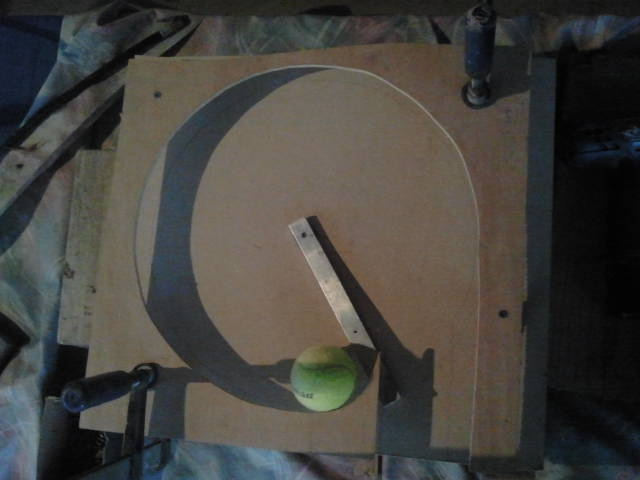
\includegraphics[width=\textwidth]{../../fig/prototyp_propeller.jpg}
		\caption{Prototyp Drehrad mit Mitnehmer}
	\end{subfigure}
	\caption{Testaufbau}
	\label{fig:drehrad_mitnehmer}
\end{figure}
